%% LaTeX template for BSc Computing for Games final year project dissertations
%% by Edward Powley
%% Games Academy, Falmouth University, UK

%% Based on:
%% bare_jrnl.tex
%% V1.4b
%% 2015/08/26
%% by Michael Shell
%% see http://www.michaelshell.org/
%% for current contact information.
%%
%% This is a skeleton file demonstrating the use of IEEEtran.cls
%% (requires IEEEtran.cls version 1.8b or later) with an IEEE
%% journal paper.
%%
%% Support sites:
%% http://www.michaelshell.org/tex/ieeetran/
%% http://www.ctan.org/pkg/ieeetran
%% and
%% http://www.ieee.org/

%%*************************************************************************
%% Legal Notice:
%% This code is offered as-is without any warranty either expressed or
%% implied; without even the implied warranty of MERCHANTABILITY or
%% FITNESS FOR A PARTICULAR PURPOSE! 
%% User assumes all risk.
%% In no event shall the IEEE or any contributor to this code be liable for
%% any damages or losses, including, but not limited to, incidental,
%% consequential, or any other damages, resulting from the use or misuse
%% of any information contained here.
%%
%% All comments are the opinions of their respective authors and are not
%% necessarily endorsed by the IEEE.
%%
%% This work is distributed under the LaTeX Project Public License (LPPL)
%% ( http://www.latex-project.org/ ) version 1.3, and may be freely used,
%% distributed and modified. A copy of the LPPL, version 1.3, is included
%% in the base LaTeX documentation of all distributions of LaTeX released
%% 2003/12/01 or later.
%% Retain all contribution notices and credits.
%% ** Modified files should be clearly indicated as such, including  **
%% ** renaming them and changing author support contact information. **
%%*************************************************************************


\documentclass[journal]{IEEEtran}

\usepackage{graphicx}
% to embed the file `myreferences.bib` in your `.tex` file
% Insert additional usepackage commands here


\begin{document}
%
% paper title
% Titles are generally capitalized except for words such as a, an, and, as,
% at, but, by, for, in, nor, of, on, or, the, to and up, which are usually
% not capitalized unless they are the first or last word of the title.
% Linebreaks \\ can be used within to get better formatting as desired.
% Do not put math or special symbols in the title.
\title{How Effective can an Adaptive AI Built With Predefined Expert Strategies be Against Competition Grade AI?}
%
%
% author name
\author{\IEEEauthorblockN{James Hellman\\}
\IEEEauthorblockA{Falmouth Games Academy\\
UK, Falmouth 1506530\\
Email: jh182233@falmouth.ac.uk\\}
}

% The paper headers -- please do not change these, but uncomment one of them as appropriate
% Uncomment this one for COMP320
\markboth{COMP320: Research Review and Proposal}{COMP320: Research Review and Proposal}
% Uncomment this one for COMP360
% \markboth{COMP360: Dissertation}{COMP360: Dissertation}

% make the title area
\maketitle

% As a general rule, do not put math, special symbols or citations
% in the abstract or keywords.
\begin{abstract}
Effective macro-management (the ability to create armies and expand bases), is essential to obtaining victory in Real-Time Strategy (RTS), in the research community many AI's have been created to handle this. One method is to use a design approach to create what is known as build orders, many of these build orders take from expert strategies used by real people in high ranking tournaments. Build orders can be ridged during games leaving little room for adaptation to the opponents strategy. In this paper a collection of build orders will be used to create an AI capable of interchanging these build orders to effectively counter several strategies. An assumption is made here that the AI will only be effective in the early stages of the game and will be outmanoeuvred in late-game stages. The effectiveness of this AI will be its time survived, and winning state.
\end{abstract}

\section{Introduction}
\IEEEPARstart{A}{I}  \cite{AIBook} \cite{Survey} 

\section{StarCraft}
\IEEEPARstart{S}{tarCraft} is an RTS game developed by Blizzard Entertainment \cite{Blizzard}, and released in 1998. Later that year StarCraft: Brood War was released and took hold as one of the greatest RTS games in gaming history, it was and is still large in the e-sports community. StarCraft 2: Wings of Liberty was released much later in 2010, with most of the game mechanics the same other than balance changes, the user interface (UI) was kept the same just with a visual overhaul. The premise of StarCraft is to gather resources, build a base, and build an army to then use to destroy an enemies base and army, during playtime there are also many upgrades available for these units to give them the edge over an enemy who did not spend the time acquiring them. There are many ways of doing this each player with a different order of building their armies/bases commonly referred to as their "Build Order" \cite{BuildOrder}. Build orders only refer to a players macro-management, whereas in StarCraft Micro-management is a huge part of the game, as those with greater control over individual units can better outmanoeuvre their opponent, and thus defeat them. This paper will be focusing on the macro-management portion of the game with a greater focus on the build order and the choosing of strategies rather than individual control of the units.

\section{Related Work}
In the StarCraft research community there are many different methods of AI creation. Some focus on micro-management like S. Liu et al \cite{EffectiveMicro} that uses a Genetic Algorithm (GA) and others that focus on macro-management looking at the build order like N. Justesen et al \cite{OnlineEvo}. Many of these research methods are cross depended and utilise more than one method for example, D. Churchill et al \cite{Agents} created the UAlbertaBot, which was intended to automate both build order planning and unit control. Though this paper is focusing on the planning aspect with an implementation of "either a Bayesian or other prediction algorithm" there are many other ways of creating an effective AI.

\subsection{Datasets}
A Dataset can be a collection of any data, for game AI a dataset can consist of thousands of replays with millions of game frames, and player actions\cite{Dataset}. This information can then put together to create a full game-state which allows for machine learning tasks \cite{Dataset17}. In AI research, datasets can be used in many approaches of development, one such use is to recreate game-states and evaluate them for prediction in realistic conditions \cite{SpecialTactics}.

 
\subsection{Bayesian Approaches}
Bayesian approaches are based on Bayes' Theorem, a calculation of probability or also known as a probabilistic model \cite{BayesianAI}. In papers by G. Synnaeve et al \cite{UnitsControl}\cite{SpecialTactics} they create an AI that controls units individually, they do this by using uncertainty which instead of asking where a unit might be, it makes rough estimations and acts upon that. Another use for the Bayesian approach is to predict strategies, by creating a probabilistic model that after learning from replays can predict an opponents strategy and adapt accordingly \cite{Bayesian}. A major downfalls of Bayesian Approaches is that it can be computationally intense to calculate.

\subsection{Micro-Management}
Micro management is a fundamental side of StarCraft game-play and many papers have their own approach to this aspect of RTS \cite{SOMA}\cite{EffectiveMicro}\cite{Swarm}\cite{MM}\cite{SpecialTactics}\cite{UnitsControl}. Many of these approaches us either Genetic Algorithms (GA) or Evolutionary Algorithms (EA) \cite{SOMA}\cite{EffectiveMicro}\cite{Swarm}, while others observe replays and apply a Monte-Carlo method to create data for practice use \cite{MM}. But most of these methods have one thing in common, they all use a version of machine learning \cite{Survey}.

\subsection{Prediction}
On a higher strategic level the prediction of the opponents strategy is an prominent approach used in research \cite{DataMine}\cite{Bayesian}\cite{Scouting}\cite{ReplayPred}. This type of research relies on the use of replays and machine learning to help the AI accurately predict a strategy, these do rely on the quantity and quality of replays used for the learning process\cite{DataMine}\cite{Bayesian}\cite{ReplayPred}. Another method for prediction is scouting alongside machine learning, this eliminates the need for replay observation and allows for a more real-time prediction \cite{Scouting}. Though this method does still require several games to be played before the AI can begin to have an accurate prediction.

\subsection{Full Game Play}
Many papers try to create an AI capable of handling all aspects of an RTS \cite{Agents}\cite{Hierarchical}\cite{HumanLevel}\cite{SCAIL}. These AI's tend to take several methods that have been created in other research and combining them to form a new AI \cite{Agents}. Another use for the full game play AI is to try and create a "Human-Like" AI, which can mimic the play-style of an expert human player though the current AI's are limited in this as players reported that the AI's used unusual unit movements or building placement \cite{EvalHuman}.

\subsection{Neural Networks}
Neural Networking are computational models loosely based on the functioning of biological brains \cite{Deep}. Given an input it computes an output by using a large number of neural units, in StarCraft it can be used to predict strategies or in the case of StarCraft 2 with its new architecture it can be used for full game-play. Using a neural network would be impractical for the purpose of this paper as ti would take many months to train.

\subsection{Planning}
Planning in StarCraft usually deals with the build order that the AI will use usually only dealing with macro-management. There are several different ways to use a build order, some will use a static build order that will not change throughout the game \cite{Swen}, and the more popular route is to allow the AI to jump between build orders during play-time, another term is Reactive Planning \cite{Fuzzy}\cite{OnlineEvo}\cite{GoalDriven}. there has been some work on creating the build orders on the fly by finding out that most optimal method of gathering resource and building units \cite{BuildOrder}. Planning is perhaps the most optimal approach to creating an AI as there is little real-time calculations to make. Through the use of Parallel-rooted Ordered Slip-stack Hierarchical (POSH) reactive plans \cite{POSH}, you can iteratively design AI prototypes quickly \cite{Swen}.

\section{Method}
This paper will be focusing on the implementation of an AI with pre-built build orders and their counters taken from Liquipedia \cite{Liquid}, a website dedicated to StarCraft, on the there they have a collection of strategies that are free to use in any capacity. Building upon these build orders the experiment will also include a method for swapping between the orders at any point, to know when to do this, the AI will scout the map in search of the opponent and compare their current building to its stored build orders and find an appropriate counter. The issue with this method is that in late game the AI will struggle to decide which build order to continue. 

\subsection{Tools}
There are several tools that will be using in this experiment, these include The Brood War Application Programming Interface (BWAPI), POSH tools, specifically POSH Sharp which is an interface that uses cSharp instead of C++, and the ABODE editing software which uses POSH plans to create Behaviour Oriented Design's for AI's. 

BWAPI \cite{BWAPI} is a open source software that creates an interface for a custom AI to use to communicate with the game. BWAPI deliberately does not give access to all the games information \cite{POSH}, limiting the AI to only be able to have information on the enemy if there is no Fog-of-War currently covering them, as well as the size of the map and base locations. This prevents custom AI's from cheating and ensures a fair game, though this could be considered a plus as it means that the developers of these AI's do not need to worry about using information that could cause their AI to cheat. Though this does mean hat all the AI's must work in an imperfect environment which forces the AI to have to scout for information.

The POSH tool as seen in Figure 1, is a visual planning tool that allows for hierarchy of actions with associated triggers.

\begin{figure}[h]
	\centering
	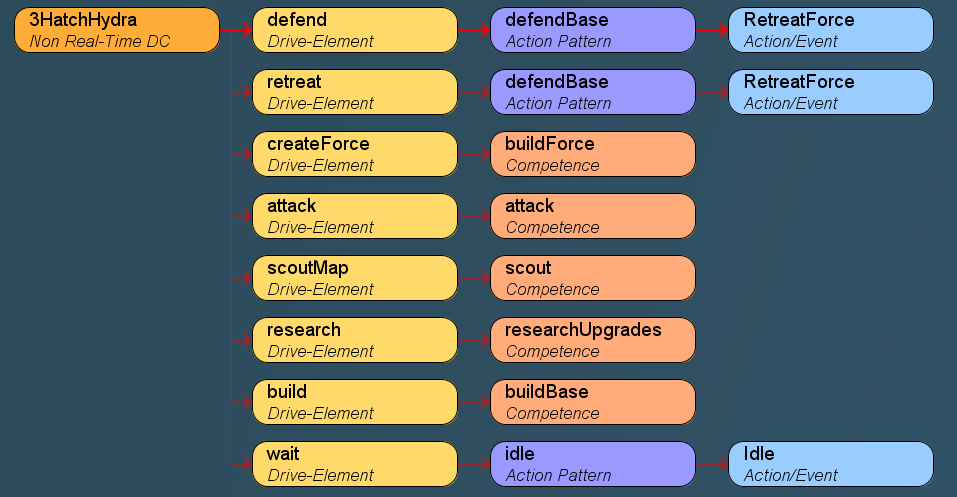
\includegraphics[width=0.5\textwidth]{POSH}
	\caption{POSH plan for the Three Hatch Hydra build plan inside the ABODE editor.}
	\label{fig:mesh1}
\end{figure}
\newpage
How to measure?
% references section

\bibliographystyle{IEEEtran}
\bibliography{references}

% Appendices


% that's all folks
\end{document}
